\documentclass[border=0mm]{standalone}

\usepackage{tikz}
\usepackage{fix-cm} 

\usetikzlibrary{calc}
\usetikzlibrary{external}

\newcommand*{\width }{65mm}%
\newcommand*{\height}{110mm}%
\newcommand*{\hwd   }{\width/2}%
\newcommand*{\hht   }{\height/2}%
\newcommand*{\stp   }{\width/6}
\newcommand*{\stb   }{\stp*1.4142}   

\makeatletter
\newcommand\HUGE{\@setfontsize\Huge{50}{60}}
\makeatother

\tikzexternalize

\begin{document}
    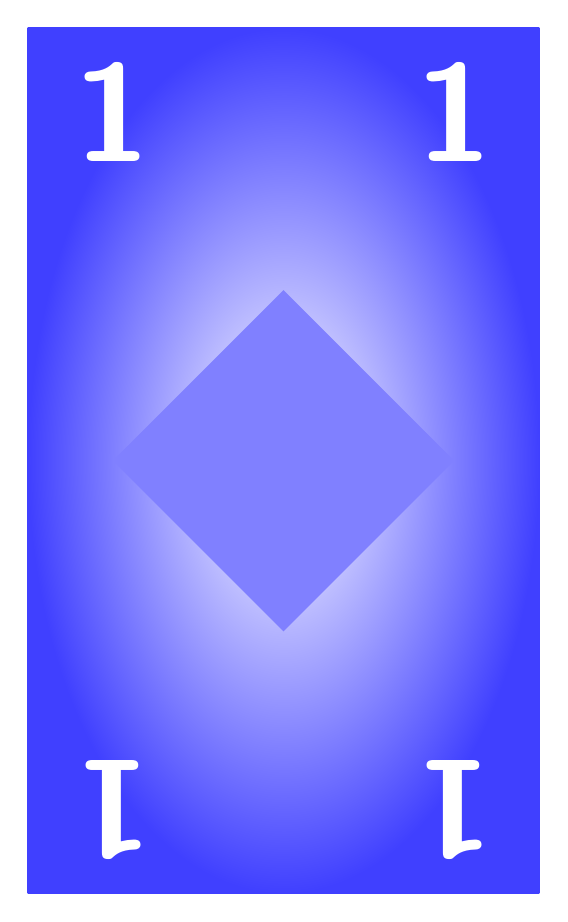
\begin{tikzpicture}[font=\sffamily]
    	\shade [ inner color = white, outer color = blue!75!white, shading=radial] (-\hwd,-\hht) -- ++(0,\height) -- ++(\width,0) -- ++(0,-\height) -- cycle;
        \node [rotate= 00, text=white] at ( \hwd-\stp, \hht-\stp) {\textbf{\HUGE 1}};
        \node [rotate= 00, text=white] at (-\hwd+\stp, \hht-\stp) {\textbf{\HUGE 1}};
        \node [rotate=180, text=white] at ( \hwd-\stp,-\hht+\stp) {\textbf{\HUGE 1}};
        \node [rotate=180, text=white] at (-\hwd+\stp,-\hht+\stp) {\textbf{\HUGE 1}};
        \draw [rotate=45, fill=blue!50!, draw = none] (-\stb,-\stb) rectangle (\stb,\stb);
        %\draw [fill=blue!25!, draw = none] (-\stp,-\stp) rectangle (\stp,\stp);
    \end{tikzpicture}
    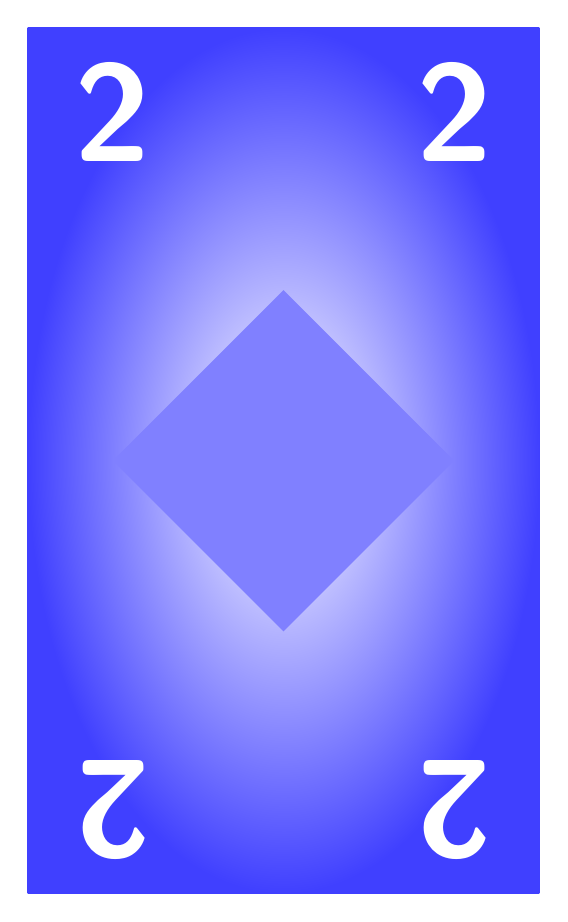
\begin{tikzpicture}[font=\sffamily]
    	\shade [ inner color = white, outer color = blue!75!white, shading=radial] (-\hwd,-\hht) -- ++(0,\height) -- ++(\width,0) -- ++(0,-\height) -- cycle;
        \node [rotate= 00, text=white] at ( \hwd-\stp, \hht-\stp) {\textbf{\HUGE 2}};
        \node [rotate= 00, text=white] at (-\hwd+\stp, \hht-\stp) {\textbf{\HUGE 2}};
        \node [rotate=180, text=white] at ( \hwd-\stp,-\hht+\stp) {\textbf{\HUGE 2}};
        \node [rotate=180, text=white] at (-\hwd+\stp,-\hht+\stp) {\textbf{\HUGE 2}};
        \draw [rotate=45, fill=blue!50!, draw = none] (-\stb,-\stb) rectangle (\stb,\stb);
        %\draw [fill=blue!25!, draw = none] (-\stp,-\stp) rectangle (\stp,\stp);
    \end{tikzpicture}
    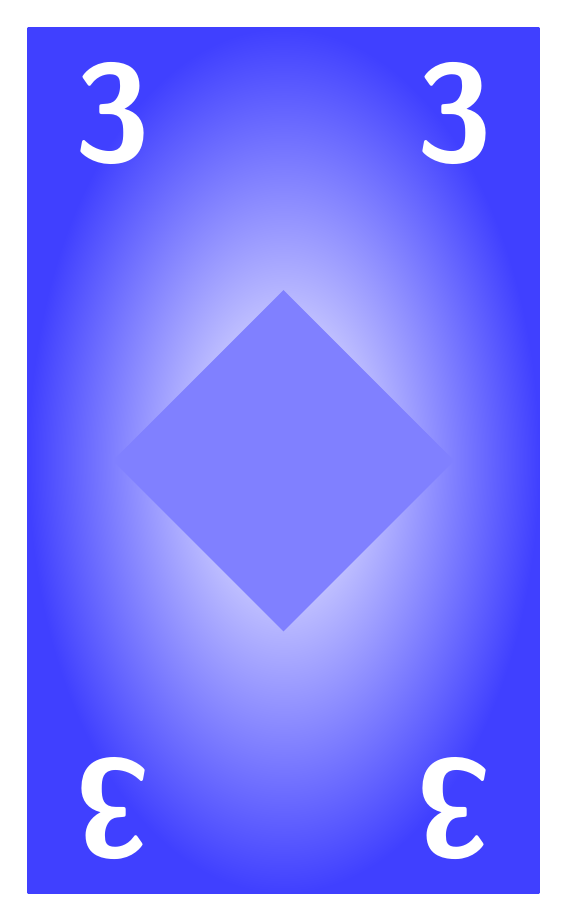
\begin{tikzpicture}[font=\sffamily]
    	\shade [ inner color = white, outer color = blue!75!white, shading=radial] (-\hwd,-\hht) -- ++(0,\height) -- ++(\width,0) -- ++(0,-\height) -- cycle;
        \node [rotate= 00, text=white] at ( \hwd-\stp, \hht-\stp) {\textbf{\HUGE 3}};
        \node [rotate= 00, text=white] at (-\hwd+\stp, \hht-\stp) {\textbf{\HUGE 3}};
        \node [rotate=180, text=white] at ( \hwd-\stp,-\hht+\stp) {\textbf{\HUGE 3}};
        \node [rotate=180, text=white] at (-\hwd+\stp,-\hht+\stp) {\textbf{\HUGE 3}};
        \draw [rotate=45, fill=blue!50!, draw = none] (-\stb,-\stb) rectangle (\stb,\stb);
        %\draw [fill=blue!25!, draw = none] (-\stp,-\stp) rectangle (\stp,\stp);
    \end{tikzpicture}
    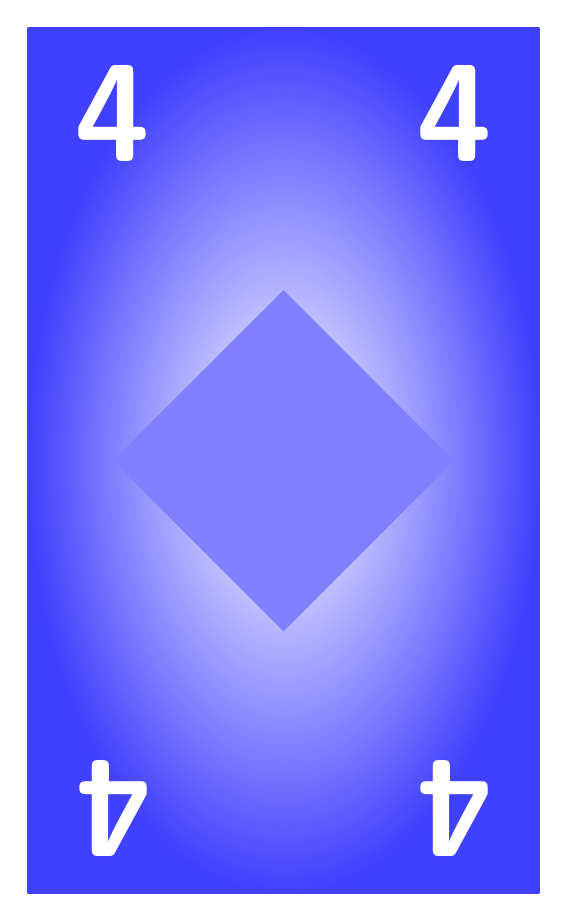
\begin{tikzpicture}[font=\sffamily]
    	\shade [ inner color = white, outer color = blue!75!white, shading=radial] (-\hwd,-\hht) -- ++(0,\height) -- ++(\width,0) -- ++(0,-\height) -- cycle;
        \node [rotate= 00, text=white] at ( \hwd-\stp, \hht-\stp) {\textbf{\HUGE 4}};
        \node [rotate= 00, text=white] at (-\hwd+\stp, \hht-\stp) {\textbf{\HUGE 4}};
        \node [rotate=180, text=white] at ( \hwd-\stp,-\hht+\stp) {\textbf{\HUGE 4}};
        \node [rotate=180, text=white] at (-\hwd+\stp,-\hht+\stp) {\textbf{\HUGE 4}};
        \draw [rotate=45, fill=blue!50!, draw = none] (-\stb,-\stb) rectangle (\stb,\stb);
        %\draw [fill=blue!25!, draw = none] (-\stp,-\stp) rectangle (\stp,\stp);
    \end{tikzpicture}
    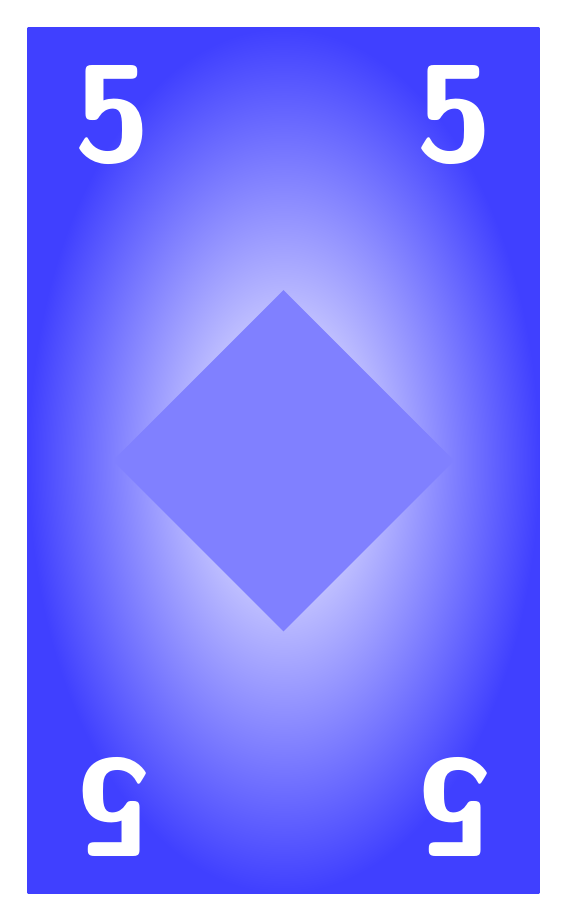
\begin{tikzpicture}[font=\sffamily]
    	\shade [ inner color = white, outer color = blue!75!white, shading=radial] (-\hwd,-\hht) -- ++(0,\height) -- ++(\width,0) -- ++(0,-\height) -- cycle;
        \node [rotate= 00, text=white] at ( \hwd-\stp, \hht-\stp) {\textbf{\HUGE 5}};
        \node [rotate= 00, text=white] at (-\hwd+\stp, \hht-\stp) {\textbf{\HUGE 5}};
        \node [rotate=180, text=white] at ( \hwd-\stp,-\hht+\stp) {\textbf{\HUGE 5}};
        \node [rotate=180, text=white] at (-\hwd+\stp,-\hht+\stp) {\textbf{\HUGE 5}};
        \draw [rotate=45, fill=blue!50!, draw = none] (-\stb,-\stb) rectangle (\stb,\stb);
        %\draw [fill=blue!25!, draw = none] (-\stp,-\stp) rectangle (\stp,\stp);
    \end{tikzpicture}
    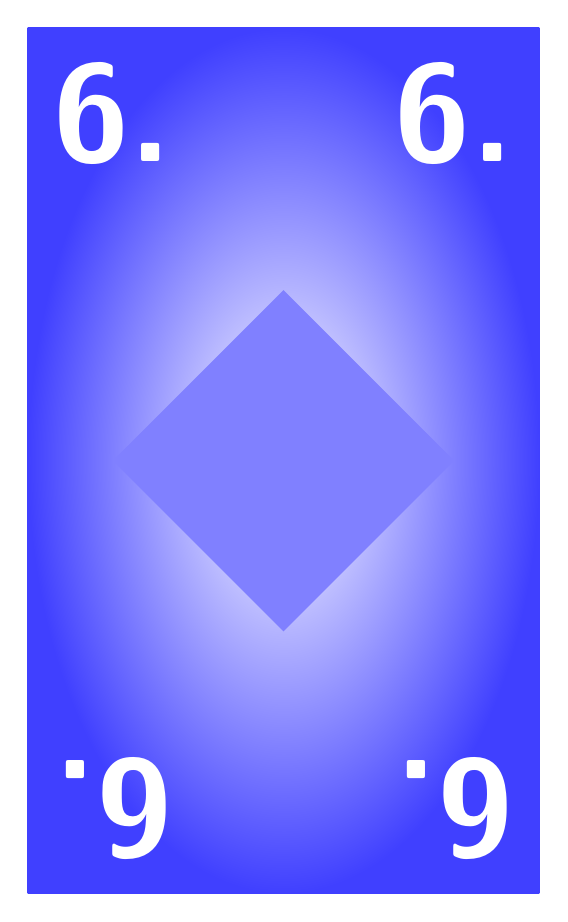
\begin{tikzpicture}[font=\sffamily]
    	\shade [ inner color = white, outer color = blue!75!white, shading=radial] (-\hwd,-\hht) -- ++(0,\height) -- ++(\width,0) -- ++(0,-\height) -- cycle;
        \node [rotate= 00, text=white] at ( \hwd-\stp, \hht-\stp) {\textbf{\HUGE 6.}};
        \node [rotate= 00, text=white] at (-\hwd+\stp, \hht-\stp) {\textbf{\HUGE 6.}};
        \node [rotate=180, text=white] at ( \hwd-\stp,-\hht+\stp) {\textbf{\HUGE 6.}};
        \node [rotate=180, text=white] at (-\hwd+\stp,-\hht+\stp) {\textbf{\HUGE 6.}};
        \draw [rotate=45, fill=blue!50!, draw = none] (-\stb,-\stb) rectangle (\stb,\stb);
        %\draw [fill=blue!25!, draw = none] (-\stp,-\stp) rectangle (\stp,\stp);
    \end{tikzpicture}
    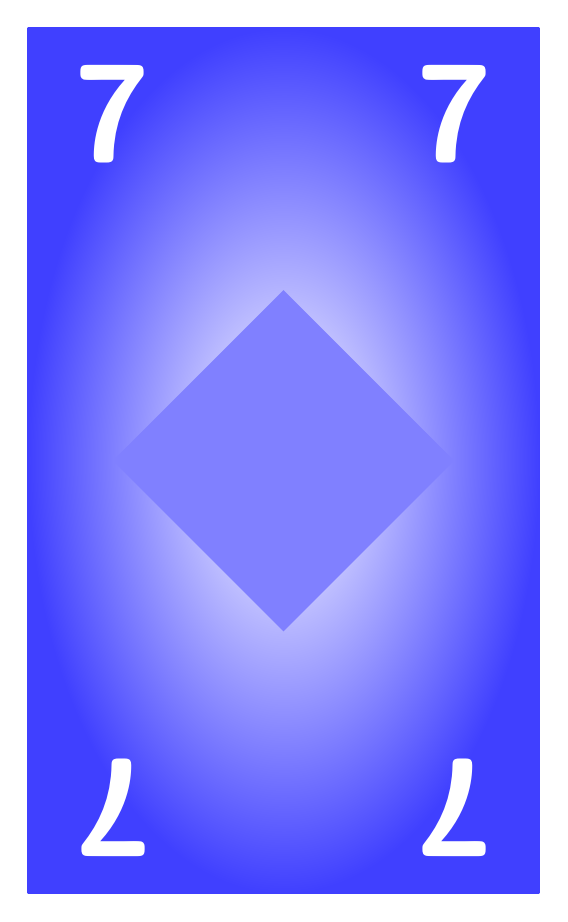
\begin{tikzpicture}[font=\sffamily]
    	\shade [ inner color = white, outer color = blue!75!white, shading=radial] (-\hwd,-\hht) -- ++(0,\height) -- ++(\width,0) -- ++(0,-\height) -- cycle;
        \node [rotate= 00, text=white] at ( \hwd-\stp, \hht-\stp) {\textbf{\HUGE 7}};
        \node [rotate= 00, text=white] at (-\hwd+\stp, \hht-\stp) {\textbf{\HUGE 7}};
        \node [rotate=180, text=white] at ( \hwd-\stp,-\hht+\stp) {\textbf{\HUGE 7}};
        \node [rotate=180, text=white] at (-\hwd+\stp,-\hht+\stp) {\textbf{\HUGE 7}};
        \draw [rotate=45, fill=blue!50!, draw = none] (-\stb,-\stb) rectangle (\stb,\stb);
        %\draw [fill=blue!25!, draw = none] (-\stp,-\stp) rectangle (\stp,\stp);
    \end{tikzpicture}
    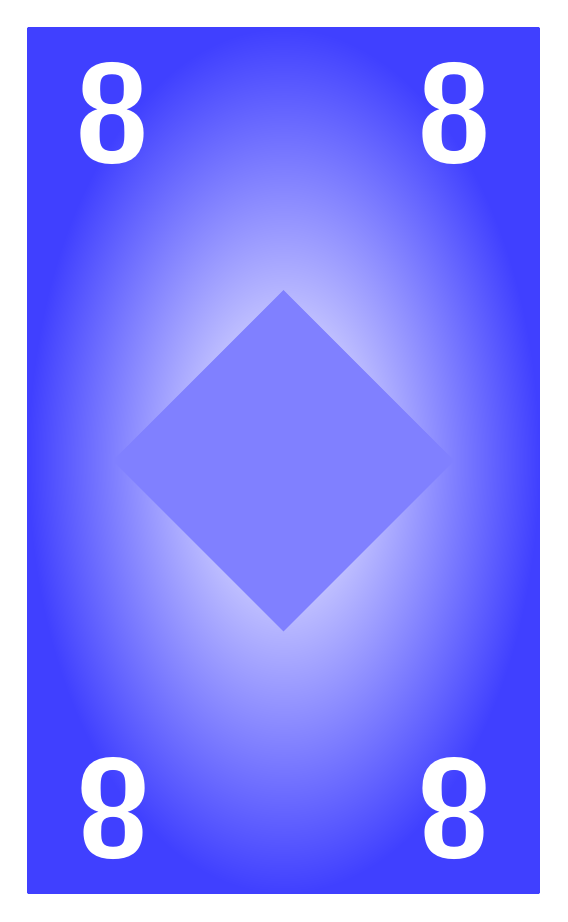
\begin{tikzpicture}[font=\sffamily]
    	\shade [ inner color = white, outer color = blue!75!white, shading=radial] (-\hwd,-\hht) -- ++(0,\height) -- ++(\width,0) -- ++(0,-\height) -- cycle;
        \node [rotate= 00, text=white] at ( \hwd-\stp, \hht-\stp) {\textbf{\HUGE 8}};
        \node [rotate= 00, text=white] at (-\hwd+\stp, \hht-\stp) {\textbf{\HUGE 8}};
        \node [rotate=180, text=white] at ( \hwd-\stp,-\hht+\stp) {\textbf{\HUGE 8}};
        \node [rotate=180, text=white] at (-\hwd+\stp,-\hht+\stp) {\textbf{\HUGE 8}};
        \draw [rotate=45, fill=blue!50!, draw = none] (-\stb,-\stb) rectangle (\stb,\stb);
        %\draw [fill=blue!25!, draw = none] (-\stp,-\stp) rectangle (\stp,\stp);
    \end{tikzpicture}
    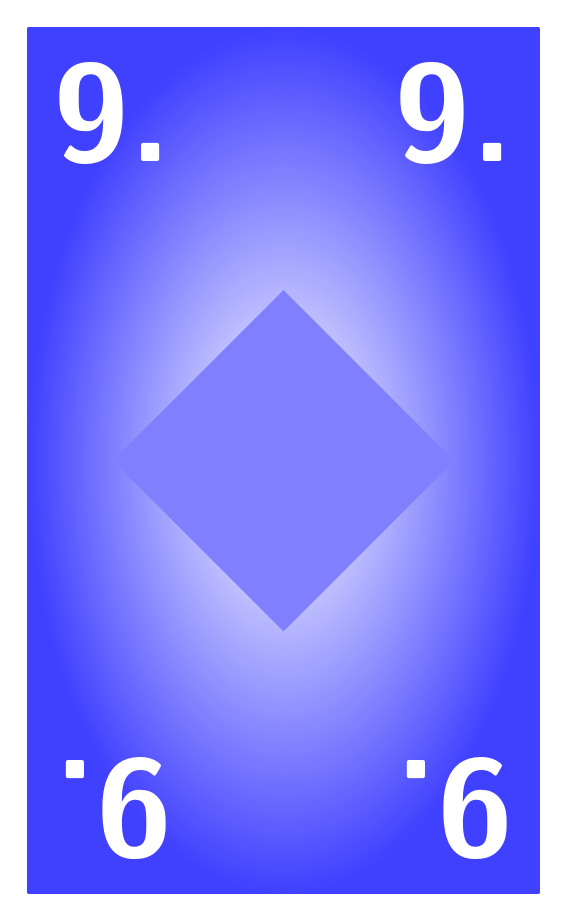
\begin{tikzpicture}[font=\sffamily]
    	\shade [ inner color = white, outer color = blue!75!white, shading=radial] (-\hwd,-\hht) -- ++(0,\height) -- ++(\width,0) -- ++(0,-\height) -- cycle;
        \node [rotate= 00, text=white] at ( \hwd-\stp, \hht-\stp) {\textbf{\HUGE 9.}};
        \node [rotate= 00, text=white] at (-\hwd+\stp, \hht-\stp) {\textbf{\HUGE 9.}};
        \node [rotate=180, text=white] at ( \hwd-\stp,-\hht+\stp) {\textbf{\HUGE 9.}};
        \node [rotate=180, text=white] at (-\hwd+\stp,-\hht+\stp) {\textbf{\HUGE 9.}};
        \draw [rotate=45, fill=blue!50!, draw = none] (-\stb,-\stb) rectangle (\stb,\stb);
        %\draw [fill=blue!25!, draw = none] (-\stp,-\stp) rectangle (\stp,\stp);
    \end{tikzpicture}
    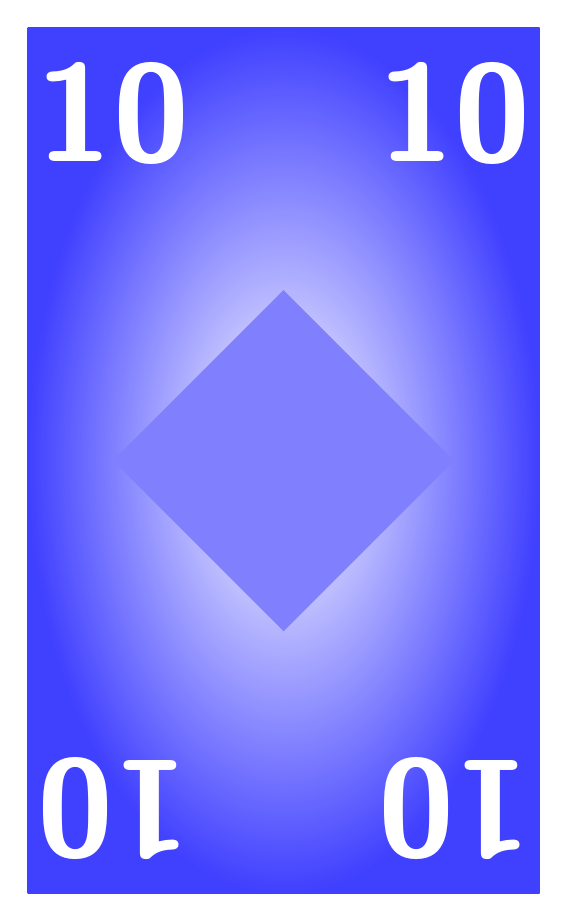
\begin{tikzpicture}[font=\sffamily]
    	\shade [ inner color = white, outer color = blue!75!white, shading=radial] (-\hwd,-\hht) -- ++(0,\height) -- ++(\width,0) -- ++(0,-\height) -- cycle;
        \node [rotate= 00, text=white] at ( \hwd-\stp, \hht-\stp) {\textbf{\HUGE 10}};
        \node [rotate= 00, text=white] at (-\hwd+\stp, \hht-\stp) {\textbf{\HUGE 10}};
        \node [rotate=180, text=white] at ( \hwd-\stp,-\hht+\stp) {\textbf{\HUGE 10}};
        \node [rotate=180, text=white] at (-\hwd+\stp,-\hht+\stp) {\textbf{\HUGE 10}};
        \draw [rotate=45, fill=blue!50!, draw = none] (-\stb,-\stb) rectangle (\stb,\stb);
        %\draw [fill=blue!25!, draw = none] (-\stp,-\stp) rectangle (\stp,\stp);
    \end{tikzpicture}
    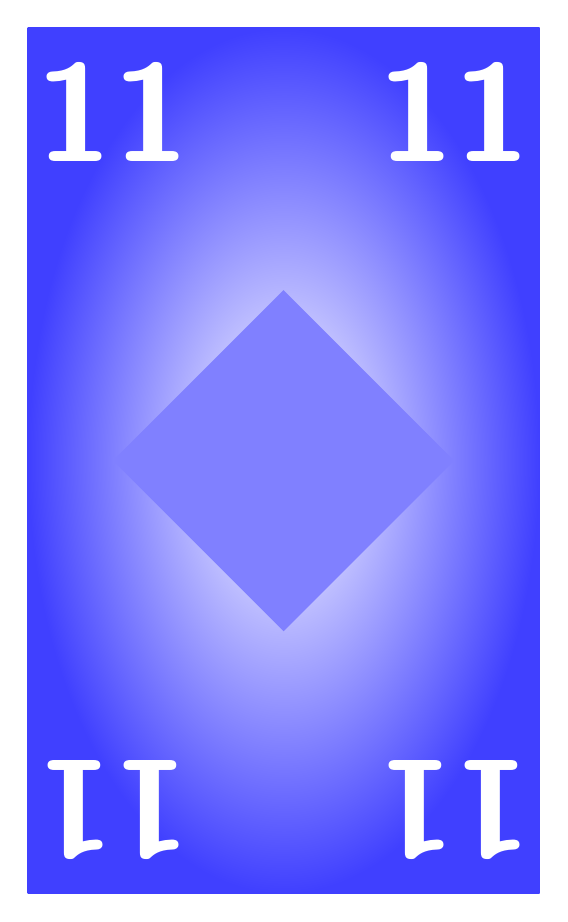
\begin{tikzpicture}[font=\sffamily]
    	\shade [ inner color = white, outer color = blue!75!white, shading=radial] (-\hwd,-\hht) -- ++(0,\height) -- ++(\width,0) -- ++(0,-\height) -- cycle;
        \node [rotate= 00, text=white] at ( \hwd-\stp, \hht-\stp) {\textbf{\HUGE 11}};
        \node [rotate= 00, text=white] at (-\hwd+\stp, \hht-\stp) {\textbf{\HUGE 11}};
        \node [rotate=180, text=white] at ( \hwd-\stp,-\hht+\stp) {\textbf{\HUGE 11}};
        \node [rotate=180, text=white] at (-\hwd+\stp,-\hht+\stp) {\textbf{\HUGE 11}};
        \draw [rotate=45, fill=blue!50!, draw = none] (-\stb,-\stb) rectangle (\stb,\stb);
        %\draw [fill=blue!25!, draw = none] (-\stp,-\stp) rectangle (\stp,\stp);
    \end{tikzpicture}
    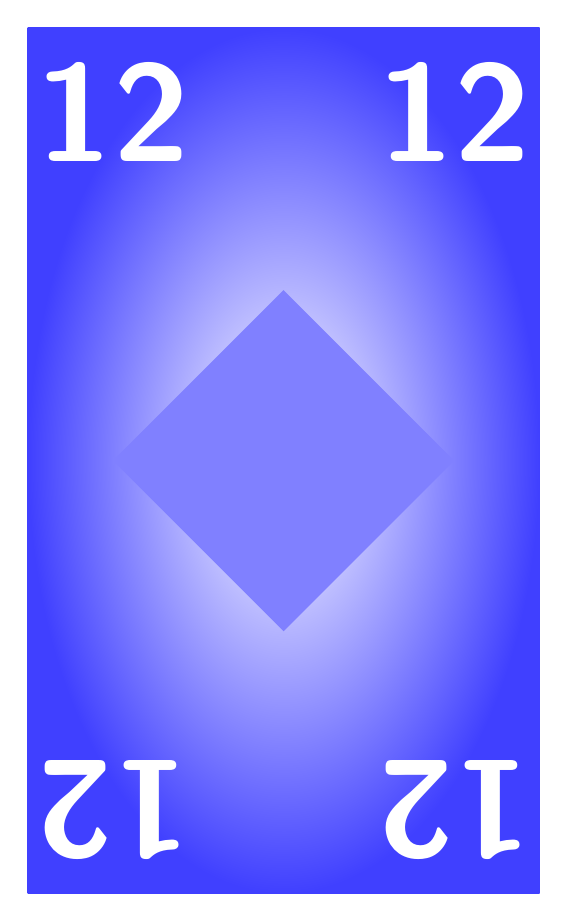
\begin{tikzpicture}[font=\sffamily]
    	\shade [ inner color = white, outer color = blue!75!white, shading=radial] (-\hwd,-\hht) -- ++(0,\height) -- ++(\width,0) -- ++(0,-\height) -- cycle;
        \node [rotate= 00, text=white] at ( \hwd-\stp, \hht-\stp) {\textbf{\HUGE 12}};
        \node [rotate= 00, text=white] at (-\hwd+\stp, \hht-\stp) {\textbf{\HUGE 12}};
        \node [rotate=180, text=white] at ( \hwd-\stp,-\hht+\stp) {\textbf{\HUGE 12}};
        \node [rotate=180, text=white] at (-\hwd+\stp,-\hht+\stp) {\textbf{\HUGE 12}};
        \draw [rotate=45, fill=blue!50!, draw = none] (-\stb,-\stb) rectangle (\stb,\stb);
        %\draw [fill=blue!25!, draw = none] (-\stp,-\stp) rectangle (\stp,\stp);
    \end{tikzpicture}
    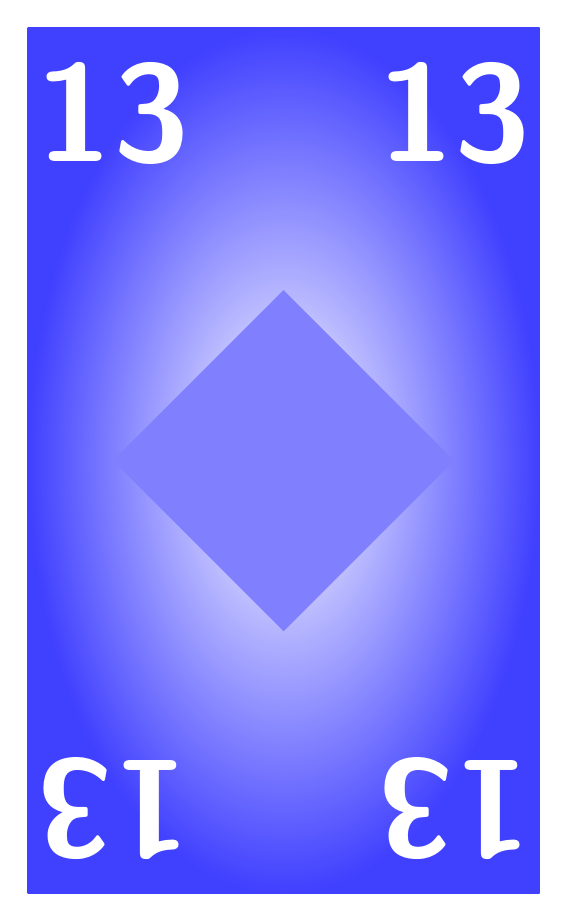
\begin{tikzpicture}[font=\sffamily]
    	\shade [ inner color = white, outer color = blue!75!white, shading=radial] (-\hwd,-\hht) -- ++(0,\height) -- ++(\width,0) -- ++(0,-\height) -- cycle;
        \node [rotate= 00, text=white] at ( \hwd-\stp, \hht-\stp) {\textbf{\HUGE 13}};
        \node [rotate= 00, text=white] at (-\hwd+\stp, \hht-\stp) {\textbf{\HUGE 13}};
        \node [rotate=180, text=white] at ( \hwd-\stp,-\hht+\stp) {\textbf{\HUGE 13}};
        \node [rotate=180, text=white] at (-\hwd+\stp,-\hht+\stp) {\textbf{\HUGE 13}};
        \draw [rotate=45, fill=blue!50!, draw = none] (-\stb,-\stb) rectangle (\stb,\stb);
        %\draw [fill=blue!25!, draw = none] (-\stp,-\stp) rectangle (\stp,\stp);
    \end{tikzpicture}
    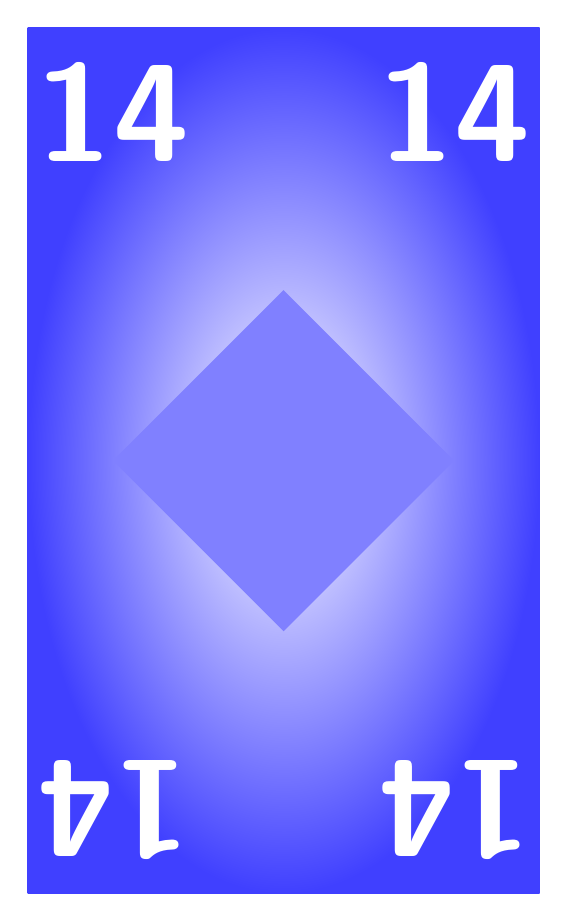
\begin{tikzpicture}[font=\sffamily]
    	\shade [ inner color = white, outer color = blue!75!white, shading=radial] (-\hwd,-\hht) -- ++(0,\height) -- ++(\width,0) -- ++(0,-\height) -- cycle;
        \node [rotate= 00, text=white] at ( \hwd-\stp, \hht-\stp) {\textbf{\HUGE 14}};
        \node [rotate= 00, text=white] at (-\hwd+\stp, \hht-\stp) {\textbf{\HUGE 14}};
        \node [rotate=180, text=white] at ( \hwd-\stp,-\hht+\stp) {\textbf{\HUGE 14}};
        \node [rotate=180, text=white] at (-\hwd+\stp,-\hht+\stp) {\textbf{\HUGE 14}};
        \draw [rotate=45, fill=blue!50!, draw = none] (-\stb,-\stb) rectangle (\stb,\stb);
        %\draw [fill=blue!25!, draw = none] (-\stp,-\stp) rectangle (\stp,\stp);
    \end{tikzpicture}
    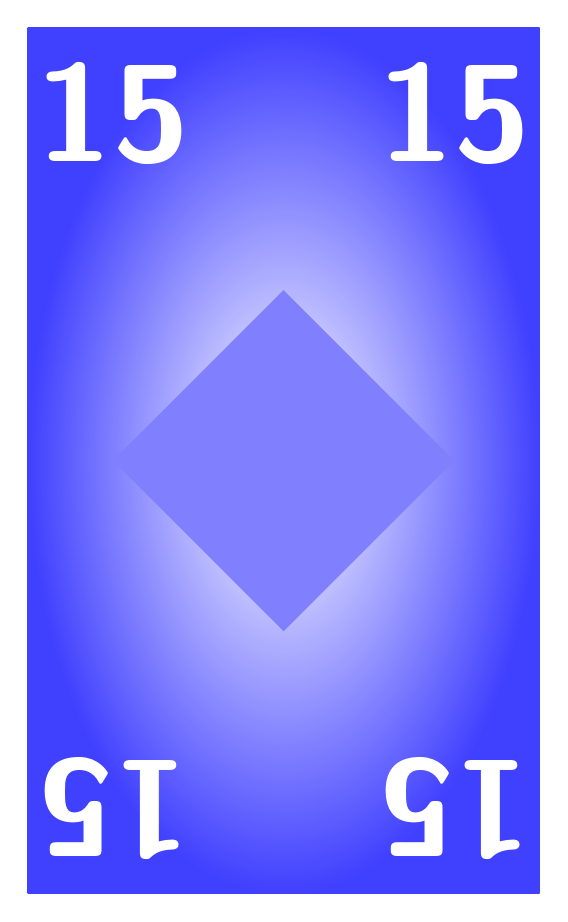
\begin{tikzpicture}[font=\sffamily]
    	\shade [ inner color = white, outer color = blue!75!white, shading=radial] (-\hwd,-\hht) -- ++(0,\height) -- ++(\width,0) -- ++(0,-\height) -- cycle;
        \node [rotate= 00, text=white] at ( \hwd-\stp, \hht-\stp) {\textbf{\HUGE 15}};
        \node [rotate= 00, text=white] at (-\hwd+\stp, \hht-\stp) {\textbf{\HUGE 15}};
        \node [rotate=180, text=white] at ( \hwd-\stp,-\hht+\stp) {\textbf{\HUGE 15}};
        \node [rotate=180, text=white] at (-\hwd+\stp,-\hht+\stp) {\textbf{\HUGE 15}};
        \draw [rotate=45, fill=blue!50!, draw = none] (-\stb,-\stb) rectangle (\stb,\stb);
        %\draw [fill=blue!25!, draw = none] (-\stp,-\stp) rectangle (\stp,\stp);
    \end{tikzpicture}
    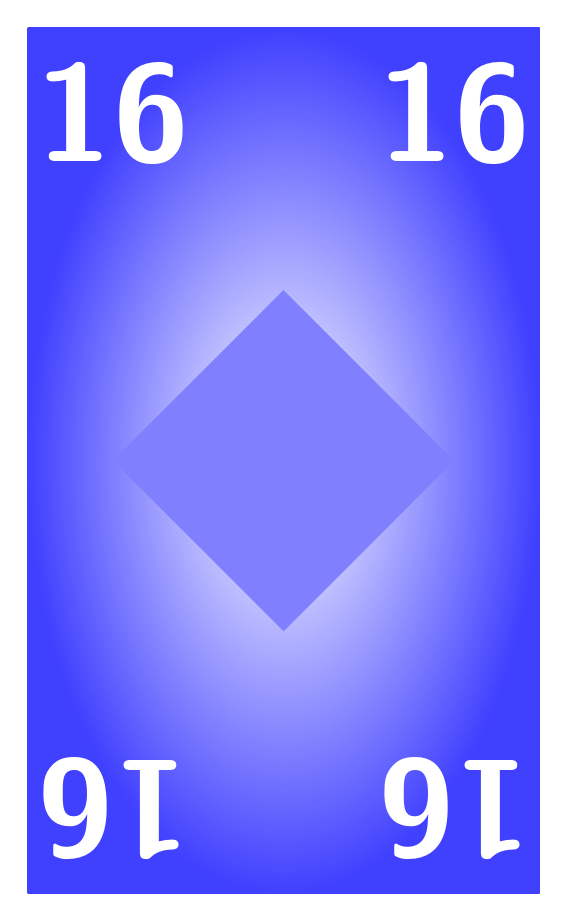
\begin{tikzpicture}[font=\sffamily]
    	\shade [ inner color = white, outer color = blue!75!white, shading=radial] (-\hwd,-\hht) -- ++(0,\height) -- ++(\width,0) -- ++(0,-\height) -- cycle;
        \node [rotate= 00, text=white] at ( \hwd-\stp, \hht-\stp) {\textbf{\HUGE 16}};
        \node [rotate= 00, text=white] at (-\hwd+\stp, \hht-\stp) {\textbf{\HUGE 16}};
        \node [rotate=180, text=white] at ( \hwd-\stp,-\hht+\stp) {\textbf{\HUGE 16}};
        \node [rotate=180, text=white] at (-\hwd+\stp,-\hht+\stp) {\textbf{\HUGE 16}};
        \draw [rotate=45, fill=blue!50!, draw = none] (-\stb,-\stb) rectangle (\stb,\stb);
        %\draw [fill=blue!25!, draw = none] (-\stp,-\stp) rectangle (\stp,\stp);
    \end{tikzpicture}
    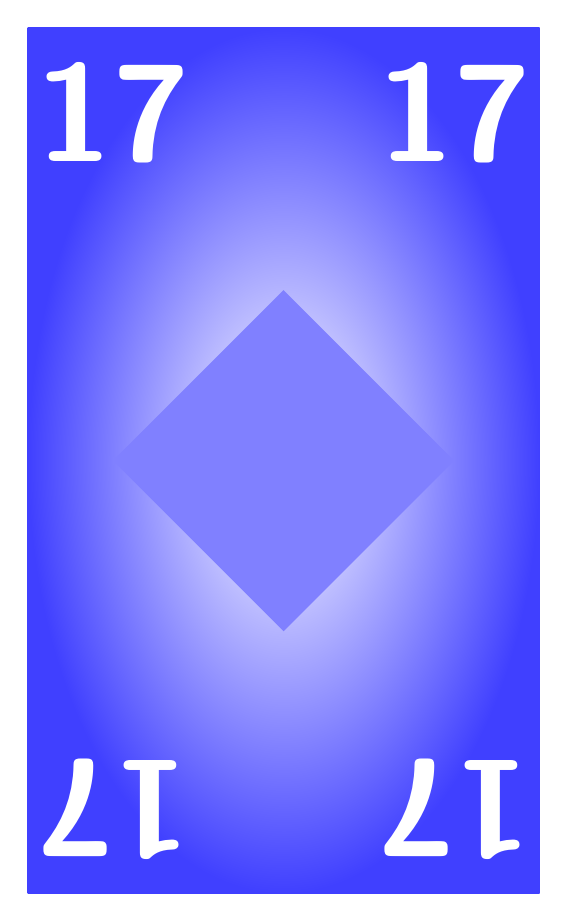
\begin{tikzpicture}[font=\sffamily]
    	\shade [ inner color = white, outer color = blue!75!white, shading=radial] (-\hwd,-\hht) -- ++(0,\height) -- ++(\width,0) -- ++(0,-\height) -- cycle;
        \node [rotate= 00, text=white] at ( \hwd-\stp, \hht-\stp) {\textbf{\HUGE 17}};
        \node [rotate= 00, text=white] at (-\hwd+\stp, \hht-\stp) {\textbf{\HUGE 17}};
        \node [rotate=180, text=white] at ( \hwd-\stp,-\hht+\stp) {\textbf{\HUGE 17}};
        \node [rotate=180, text=white] at (-\hwd+\stp,-\hht+\stp) {\textbf{\HUGE 17}};
        \draw [rotate=45, fill=blue!50!, draw = none] (-\stb,-\stb) rectangle (\stb,\stb);
        %\draw [fill=blue!25!, draw = none] (-\stp,-\stp) rectangle (\stp,\stp);
    \end{tikzpicture}
    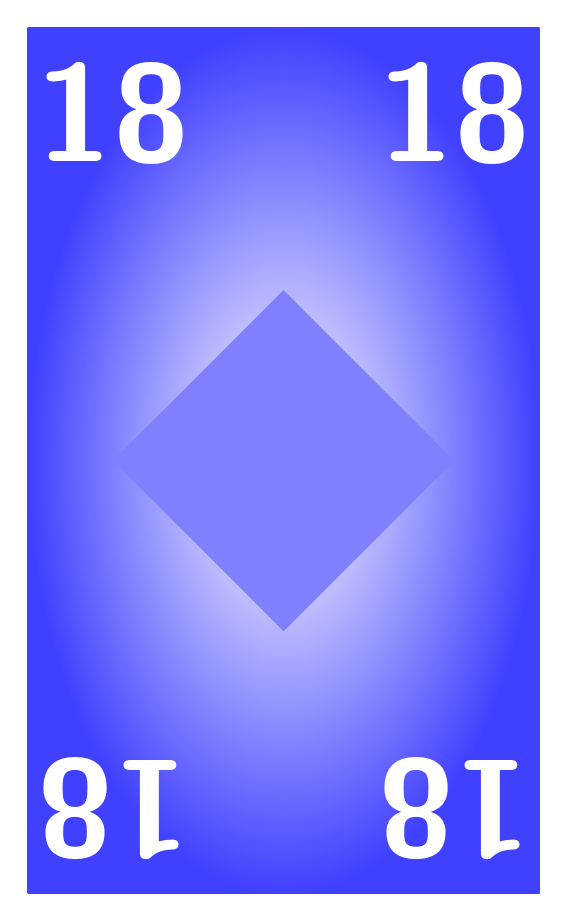
\begin{tikzpicture}[font=\sffamily]
    	\shade [ inner color = white, outer color = blue!75!white, shading=radial] (-\hwd,-\hht) -- ++(0,\height) -- ++(\width,0) -- ++(0,-\height) -- cycle;
        \node [rotate= 00, text=white] at ( \hwd-\stp, \hht-\stp) {\textbf{\HUGE 18}};
        \node [rotate= 00, text=white] at (-\hwd+\stp, \hht-\stp) {\textbf{\HUGE 18}};
        \node [rotate=180, text=white] at ( \hwd-\stp,-\hht+\stp) {\textbf{\HUGE 18}};
        \node [rotate=180, text=white] at (-\hwd+\stp,-\hht+\stp) {\textbf{\HUGE 18}};
        \draw [rotate=45, fill=blue!50!, draw = none] (-\stb,-\stb) rectangle (\stb,\stb);
        %\draw [fill=blue!25!, draw = none] (-\stp,-\stp) rectangle (\stp,\stp);
    \end{tikzpicture}
    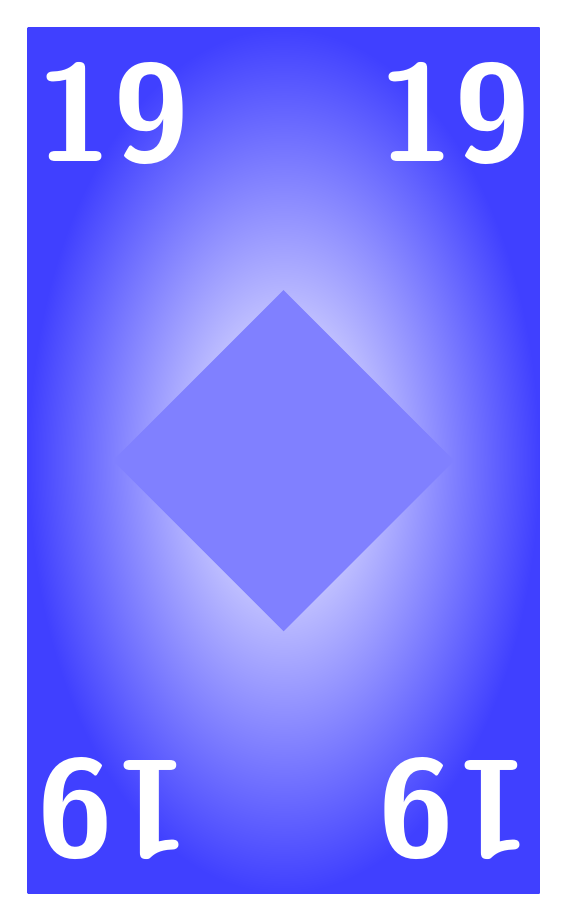
\begin{tikzpicture}[font=\sffamily]
    	\shade [ inner color = white, outer color = blue!75!white, shading=radial] (-\hwd,-\hht) -- ++(0,\height) -- ++(\width,0) -- ++(0,-\height) -- cycle;
        \node [rotate= 00, text=white] at ( \hwd-\stp, \hht-\stp) {\textbf{\HUGE 19}};
        \node [rotate= 00, text=white] at (-\hwd+\stp, \hht-\stp) {\textbf{\HUGE 19}};
        \node [rotate=180, text=white] at ( \hwd-\stp,-\hht+\stp) {\textbf{\HUGE 19}};
        \node [rotate=180, text=white] at (-\hwd+\stp,-\hht+\stp) {\textbf{\HUGE 19}};
        \draw [rotate=45, fill=blue!50!, draw = none] (-\stb,-\stb) rectangle (\stb,\stb);
        %\draw [fill=blue!25!, draw = none] (-\stp,-\stp) rectangle (\stp,\stp);
    \end{tikzpicture}

\end{document}